\documentclass[11pt]{article}

\usepackage{verbatim}
\usepackage{amsmath}
\usepackage{amssymb}
\usepackage{setspace}
\usepackage[top=1in, bottom=1in, left=1.25in, right=1.25in]{geometry}
\usepackage{subfigure}
\usepackage{graphicx}
\usepackage{cite}
\usepackage[squaren]{SIunits}
\usepackage{listings}
\usepackage{csquotes}

\setlength{\parindent}{0pt} 	% remove the silly paragraph indents

% Sample figure
%\begin{figure}[h!]
%\centering
%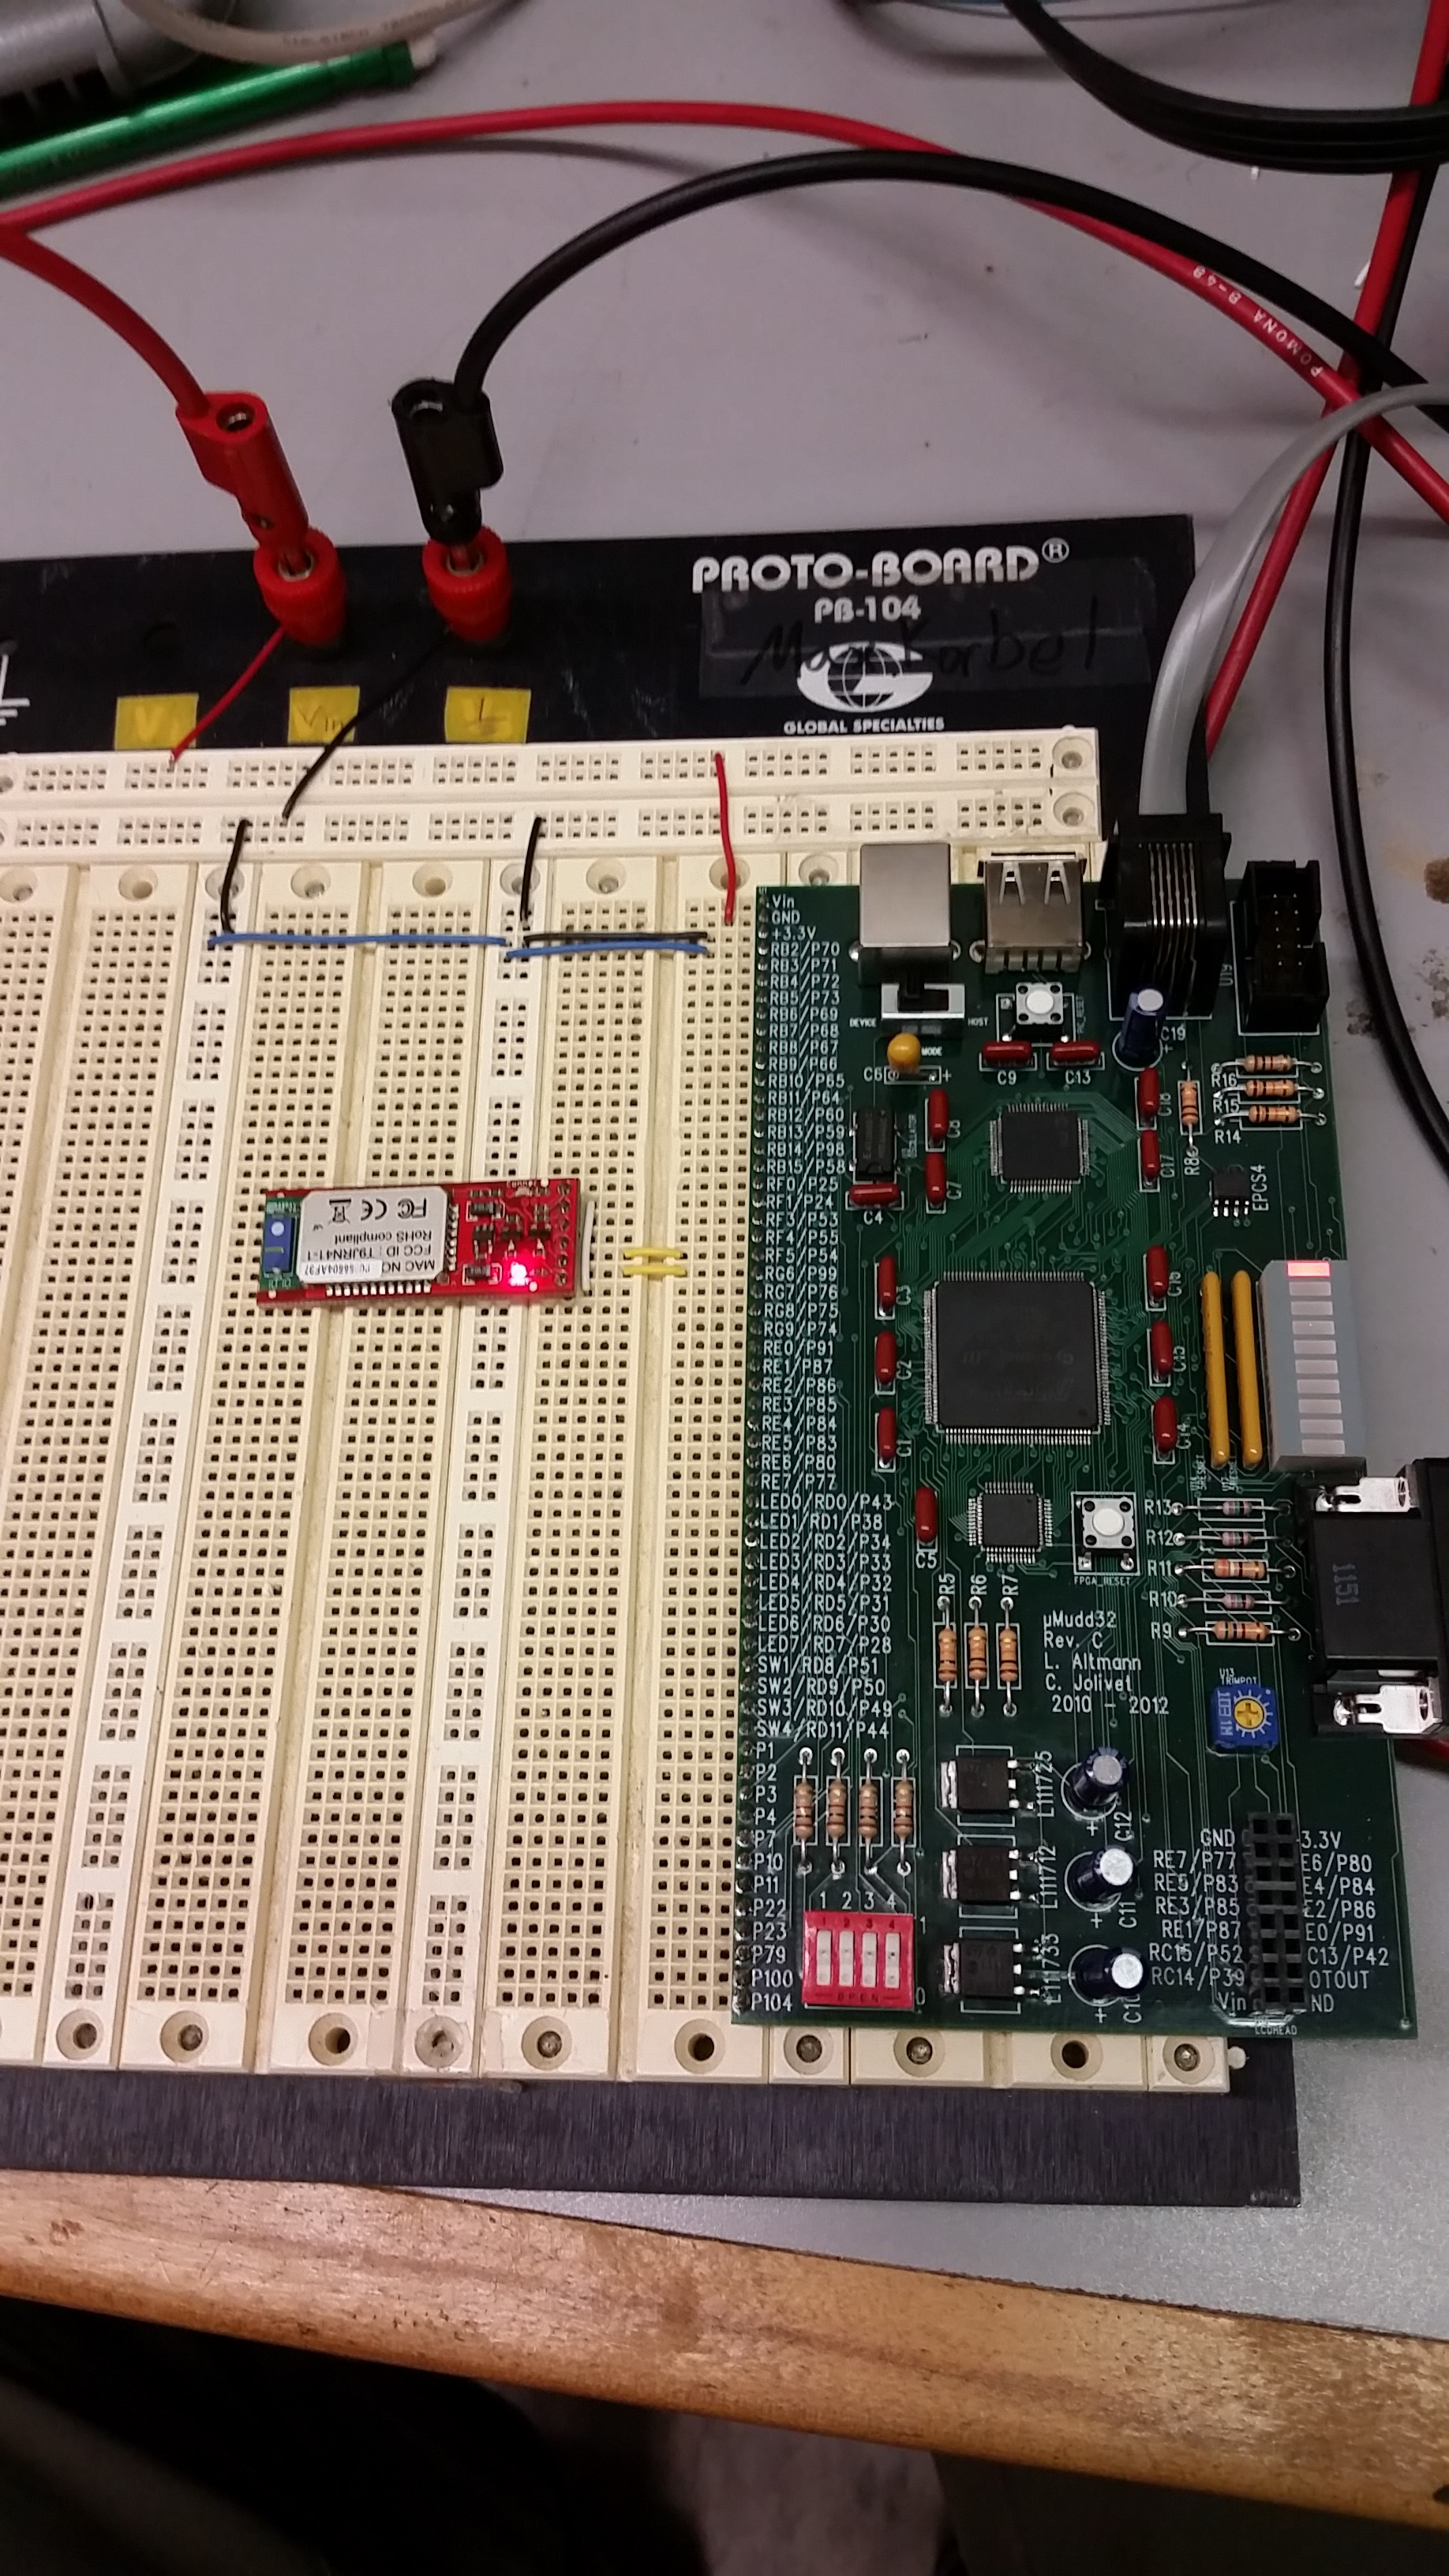
\includegraphics[scale=0.11]{board.jpg}
%\caption{The latest number entered on the keypad is displayed on the bottom display. The second latest number is displayed on the top.}
%\label{fig:board}
%\end{figure} 


\begin{document}



% ---------------------------------------
% Name section
% ---------------------------------------
\begin{flushleft}
Sherman Lam
\\E155
\\ \today
\end{flushleft}


% ---------------------------------------
% Title
% ---------------------------------------
\begin{center}
\begin{Large}
\textbf{Lab 6 Report: Wireless Calculator}
\end{Large}
\end{center}


% ---------------------------------------
% Start report
% ---------------------------------------


\section{Introduction}

In this lab, I built a wireless calculator using a PIC32 microcontroller and a bluetooth module. The module used was the Sparkfun BlueSMiRF. The pic interfaces with the BlueSMiRF through UART. On the other end of the bluetooth link is a generic USB bluetooth module connected to my laptop. I send commands over the bluetooth link through a PuTTY terminal.


\section{Design and Testing Methodology}

\subsection{Algorithm}

When strings are received, they contain a wide variety of chars. This includes numbers, mathematical symbols, and delete characters. To correctly interpret the input string correctly, I first ``clean" the string by removing all white spaces and changing the string to account for deletes. If the input was a valid mathematical expression, the cleaned expression is of form A(B)C where (B) is an operator. The expression can then be parsed and evaluated in a consistent manner. The operations handled are summation (+), subtraction (-), multiplication (*), and integer division (/).

\subsection{Hardware}
There were no special hardware connections needed. The BlueSMiRF was powered from 


\subsection{UART}


\subsection{Test Cases}
Each of the operations where tested. Various incomplete expressions were also tested to check for error handling. The program executed the operations currently and print an error when asked to evaluate invalid expressions. The test cases as well as their corresponding outputs are shown below:




You typed: 132+456
Answer: 701

You typed: 789-123
Answer: 798

You typed: 5-6
Answer: -1

You typed: 7*6
Answer: 42

You typed: 6/4
Answer: 1

You typed:14/0
Cannot divide by 0


\clearpage

\section{Technical Documentation}

\subsection{C code}

\begin{lstlisting}[numbers=left,basicstyle=\footnotesize]
/* This code plays music! The music is loaded into flash.

\end{lstlisting}



\clearpage

\clearpage

\section{Results and Discussion}



\section{Conclusion}

\subsection{Time Spent}

\begin{description}
	\item[Programming, Simulating] 6 hrs
 	\item[Writing Report] 3hrs
	\item[Total Time Spent] 9hrs
\end{description}

\subsection{Suggestions for lab}

No suggestions for the lab.

\end{document}

